\chapter{Plasma Control Systems}

\section{Overview of control systems}
The control of  plasma position, shape and current among other parameters is one of the crucial engineering problems for present and future magnetic confinement devices. The Plasma Control Systems (PCS) lead with the overall control of  fusion devices being responsible also for the  plasma configuration and scenarios algorithms \cite[Chapter~8]{PCS_2018}. Currently different PCS's are use in the tokamaks around the world. In this chapter the "DIII-D-like" PCS, the Syst\'eme de Contr\^ole Distribu\'e (SCD) and the Multi-threaded Application Real-Time executor (MARTe) will be approach, this last one being of special interest due to its extensive utilization in this work.

\subsection{DIII-D Plasma Control System}  

The DIII-D-like PCS is use in various fusion research facilities such as EAST(China), K-STAR (South Korea) and MAST (UK). Early documentation regarding the PCS in DIII-D\footnote{DIII-D is a D-shape tokamak operated by General Atomics in San Diego, California. } reefers to digitalization of analog signals transmitted to a high speed processor executing a shape control algorithm and then writing the result to a digital to analog converter for driving the controlled systems . The real-time computer used allowed to performed operations with vectors and matrices required for the plasma shape control algorithm \cite{DIIDcontrol}. Figure ~\ref{DIII1991} shows the block diagram of the DIII-D PCS 30 years ago.
\smallskip

\begin{figure}[htbp]
	\centering
	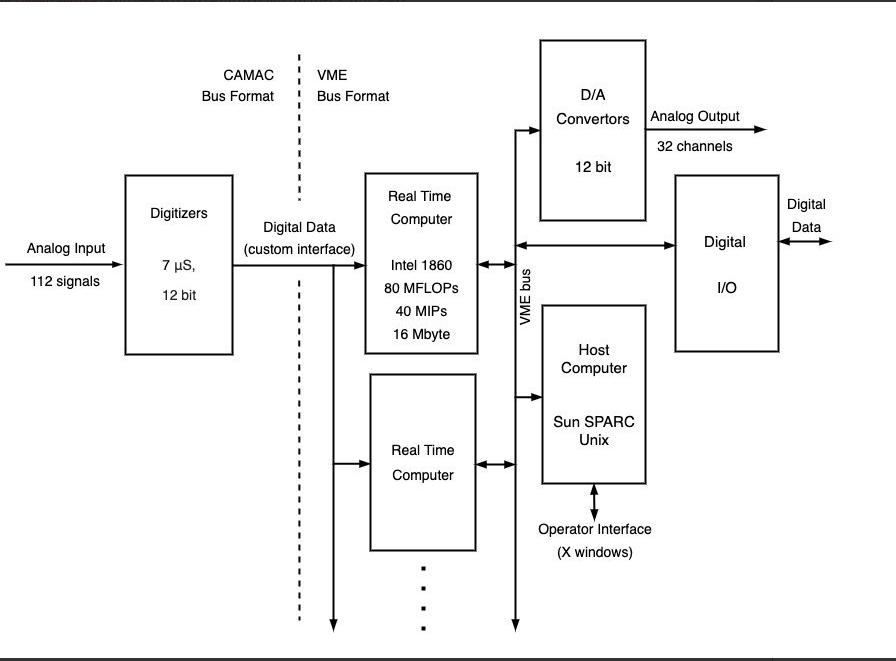
\includegraphics[width=0.65\textwidth]{Chp2/DIIDPCS_old.png}
	\caption{\label{DIII1991} DIII-D digital PCS in 1991 ~\cite{DIIDcontrol}.  }
\end{figure}

In recent years the DIII-D PCS had extensive software and hardware upgrades. The PCS actual software consists of an infrastructure library core which provides all the routines that are necessary for implementing a basic and generic control system. The current  PCS hardware configuration uses a collection of  Intel Linux based multi-processor computers running in parallel to perform the real-time analysis and feedback control ~\cite{DIIID2013}. New digitizers have been added to the real-time network to increase the number of signals acquired an to control hardware on real-time, several real-time control algorithms were added and real-time data was added to external entities such as web server.~\cite{DIIIDnew}. In the current version of the PCS, a Myricom\footnote{Myricom networks also called Myrnet are high speed networking systems used to interconnect machines to form computer clusters. } network has been replaced with a 40 Gb/sec InfiniBand\footnote{Is a network architecture from Mellanox designed to support I/O connectivity  and  reliability, availability, and serviceability Internet requirements ~\cite{MellanoxTechnologies2003}.  } network based on the Mellanox Connect-X 3\footnote{The Connect-X from the Mellanox company are Ethernet network interface cards with PCI Express.} hardware set. Figure ~\ref{DIIInew} shows the currently overall networking diagram of DIII-D PCS .


\begin{figure}[htbp]
	\centering
	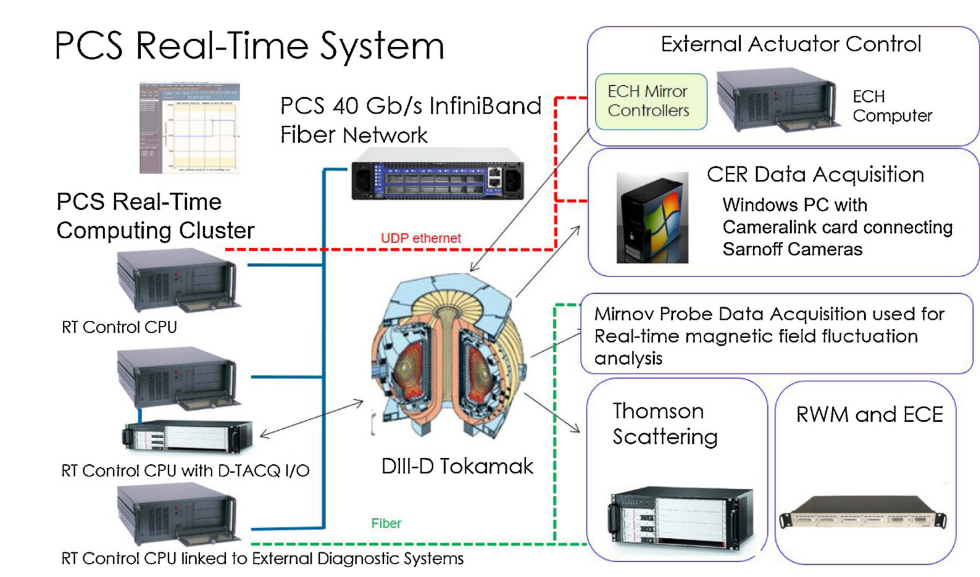
\includegraphics[width=0.65\textwidth]{Chp2/DIIIDPCSnew.PNG}
	\caption{\label{DIIInew} Actual DIII-D PCS real-time systems ~\cite{DIIIDnew}.  }
\end{figure}


\subsection{Syst\'eme de Contr\^ole Distribu\'e}

The TCV\footnote{The Tokamak \'a configuration variable (TCV) is  a medium size tokamak localized in Laussane,Switzerland. It is characterized by a highly elongated, rectangular vacuum vessel.} distributed control system uses a modular network of real time PC nodes liken by a real time network to provide feedback control over all of the actuator systems. Each node consists of a Linux PC either embedded on a Compact-PCI module or as a desktop computer with Intel CPU. A fiber optic ring network links the reflective memory (RFM) network cards in each node  \cite{TCVcntrl}.  The design of the diagnostic signal processing and control algorithms is performed in Matlab-Simulink software.  During the real-time execution  C/C++  code is generated from the Simulink and compiled  into a Linux shared library and distributed to target nodes  providing the input/output interface to the control algorithm code  ~\cite{TCVcntrl1}. Figure ~\ref{TCVcontrol} depicts the TCV SCD layout with the connectivity to diagnostics and actuators.


\begin{figure}[htbp]
	\centering
	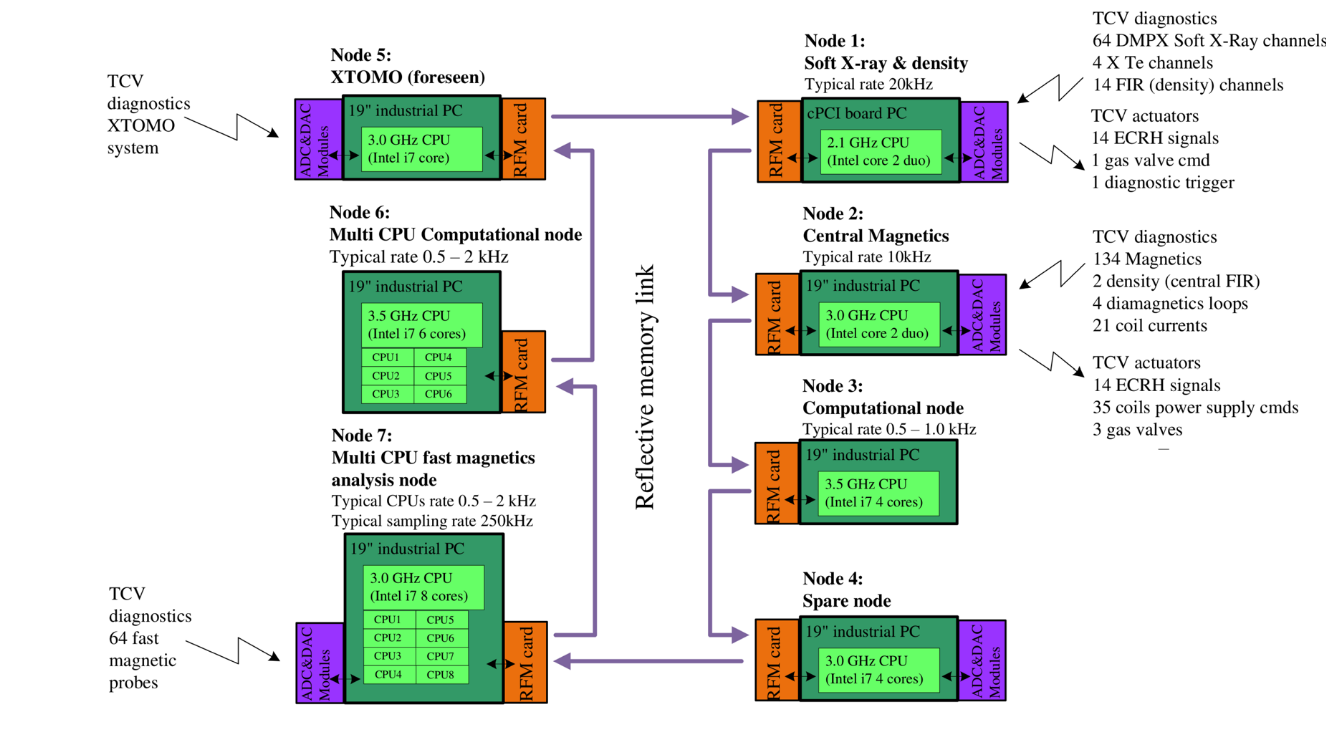
\includegraphics[width=0.65\textwidth]{Chp2/TCVcntrl1.png}
	\caption{\label{TCVcontrol} TCV SCD. Real-time network nodes connection. The nodes configurations 	are shown together with the typical diagnostic and actuator systems to which they are connected  ~\cite{TCVcntrl1}.  }
\end{figure}

\section{MARTe framework}
Regardless the nature of a real-time system the design of it is usually related to the specific requirements it has, commonly this implies to have customized hardware and software which causes a lack in modularity and portability. When systems become bigger is convenient to provide a common library containing shareable functionalities and which also allows for modular implementations. In order to deal with this the MARTe framework was designed about a decade ago. MARTe was developed in order to standardize general real-time control systems for the execution of control algorithms and is based on a multiplatform $C^{++}$ library ~\cite{Neto2010}.  Previous implementations for a  software framework similar to MARTe were developed some years before for the JET tokamak. JETRT was a software framework used to develop real-time control and data acquisition systems which laid the foundation for current MARTe framework ~\cite{JETRT}. MARTe is currently used in several tokamaks such as JET, FTU, COMPASS and ISTTOK. 

\subsection{MARTe architecture }
The unitary MARTe component is the Generic Application Module (GAM), each of the C++ programmed GAMs usually performs an specific task of the control system, the collection of interconnecting GAMs builds MARTe  \cite{Neto2011}. The GAMs  have an entry point to receive data driven configuration and a set of input and output channels to interface with other GAMs. The Dynamic Data Buffer (DDB) is a generic memory data bus where each GAM receives and produce data using DDB named channels. Usually each GAM is associated with a special function of the system like processing data of an specific diagnostic or perform some  control algorithm. MARTe hardware data interface and synchronization for inputs and outputs is performed using a special GAM called IOGAM  .


\begin{figure}[htbp]
	\centering
	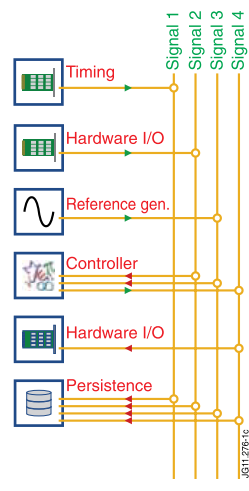
\includegraphics[width=0.35\textwidth]{Chp2/GAMs.png}
	\caption{\label{GAMs} Example of a set of GAMs connected to the DDB. Timing and hardware GAMs provide the I/O interface to the exterior, whereas a generic waveform GAM inputs the reference for a PID controller. Finally, the output is sent to a DAC and the data is stored for analysis by a collection GAM.  It should be noticed that the reference generation and the controller GAM are not aware of the changes in the data providers and data consumers.  \cite{MARTe2011}}
	
\end{figure}

\subsection{Hardware containers}

The MARTe hardware containers 


\subsection{MARTe 2.0}
Software Quality Assurance (QA) processes are being applied to the development of a new version of the MARTe framework also  called MARTe 2.0. 

\cite{MARTe2}

\section{Equilibrium and control algorithms} 
The RAPTOR (RApid Plasma Transport simulatOR) code is a model-based control-oriented code that predicts tokamak plasma profile evolution on real-time. \cite{Raptor}

\subsection{State-Space models}

\subsection{PID control}

Proportional-Integral-Derivative (PID) control 

\subsection{Multiple-Input Multiple-Output control}

Multiple-Input Multiple-Output (MIMO)